%%%%%%%%%%%%%%%%%%%%%%%%%%%%%%%%%%%%%%%%%%%%%%%%%%%%%%%%%%%%%%%
%
%\title{BioJS DAGViewer}
% 
% A paper for the BioJS series on the DAGViewer component.
%
%%%%%%%%%%%%%%%%%%%%%%%%%%%%%%%%%%%%%%%%%%%%%%%%%%%%%%%%%%%%%%%

\documentclass[10pt,a4paper,twocolumn]{article}
\usepackage{f1000_styles}
\usepackage{listings}
\usepackage{hyperref}

\definecolor{dkgreen}{rgb}{0,0.6,0}
\definecolor{gray}{rgb}{0.5,0.5,0.5}
\definecolor{mauve}{rgb}{0.58,0,0.82}

\lstdefinelanguage{JavaScript}{
  keywords={typeof, new, true, false, catch, function, return, null, catch, switch, var, if, in, while, do, else, case, break},
  keywordstyle=\color{blue}\bfseries,
  ndkeywords={class, export, boolean, throw, implements, import, this},
  ndkeywordstyle=\color{darkgray}\bfseries,
  identifierstyle=\color{black},
  sensitive=false,
  comment=[l]{//},
  morecomment=[s]{/*}{*/},
  commentstyle=\color{purple}\ttfamily,
  stringstyle=\color{red}\ttfamily,
  morestring=[b]',
  morestring=[b]"
}

\lstset{frame=tb,
  language=Javascript,
  aboveskip=3mm,
  belowskip=3mm,
  showstringspaces=false,
  columns=flexible,
  basicstyle={\small\ttfamily},
  numbers=none,
  numberstyle=\tiny\color{gray},
  keywordstyle=\color{blue},
  commentstyle=\color{dkgreen},
  stringstyle=\color{mauve},
  breaklines=true,
  breakatwhitespace=true
  tabsize=3
}

\begin{document}


\title{\textit{BioJS} DAGViewer Component \\
\small{A reusable javascript component for displaying connected graphs of information.}
}

\author[1]{Alexis Kalderimis \thanks{alex@intermine.org}}
\author[1]{Radek Štěpán \thanks{radek@intermine.org}}
\author[1]{Julie Sullivan \thanks{julie@flymine.org}}
\author[1]{Rachel Lyne \thanks{rachel@flymine.org}}
\author[1]{Michael Lyne \thanks{mike@intermine.org}}
\author[1]{Gos Micklem \thanks{g.micklem@gen.cam.ac.uk - corresponding author}}
\affil[1]{Department of Genetics and Cambridge Systems Biology Centre, Cambridge University, Downing Street, Cambridge, CB2 3EH, UK.}

\maketitle
\thispagestyle{fancy}


\begin{abstract}

The DAGViewer BioJS component is a reusable Javascript
component made available as part of the BioJS project and intended
display graphs of structured data, with a particular emphasis on
Directed Acyclic Graphs (DAGs). It enables users to
display representations of graphs of data, such as ontologies
or phylogenetic trees, in hyper-text (HTML) documents. 
This component is generic, since it is capable (given the appropriate configuration)
of displaying any kind of data which is organised as a graph.
The features of this component which are useful for examining and
filtering large and complex graphs are described.

\end{abstract}
\clearpage

\section*{Introduction}

The \emph{graph} abstract data type is an important concept in mathematics
and computer science, and is the most appropriate representation for several
classes of real world phenomena and scientific constructions. Some examples of
these include phylogenetic trees, protein-protein interaction networks and 
scientific ontologies such as the Gene Ontology ~\cite{GO} and the Sequence
ontology ~\cite{SO}. One feature of this type of data structure is that they are
much easier for humans to understand when presented as a graphical network which
preserves the structured nature of the data, than
when they are displayed flattened in tabular or list format. The component described
here is capable of displaying graphs of data, in particular Directed Acyclic Graphs (DAGs),
efficiently using Javascript to calculate the layout, and features of
modern web-browers for rendering, and is designed to integrate with other components
in the BioJS~\cite{site:biojs} project.

\subsection*{Current Tools}

A standard approach to rendering graphs visually is through Sugiyama-style 
graph drawing ~\cite{sugiyama}. This method uses heuristics to layout elements
of the network so as to minimise artifacts such as edge crossings, while keeping
related elements in close proximity to each other. A typical use of this 
alogrithm is to use a tool, such as GraphViz~\cite{graphviz}
to produce an image file which can be displayed by a number of different programs,
such as web-browsers.

This approach requires generating image files on a computer, either on demand
or through batch-preprocessing, and then sending them out over the network to
a suitable display device. This requires that any group wishing to view graphical
network analysis need have access to the resources and expertise to manage either
a server capable of dynamically generating such images, or to preproduce the
images required in advance. In either case, user interaction is very limited.

Modern web-browsers have advanced to the point where it is now practical to
calculate layouts for graphs of moderate size (in the order of around 200 to 500
nodes, depending on density of connections) and render them in a dynamic hyper-text
page, using tools such as Javascript and Scaled Vector Graphics (SVG). This accounts
for the great majority of networks that one might want to visualise, particularly
since networks of greater information densities are very difficult for humans to
interpret event when rendered. We have taken advantage of the opportunity afforded
by modern browser tools to produce a generic network display tool suitable for a
variety of scientific purposes and providing a much greater degree of customisation,
interaction and flexibility than typical image generation approaches.

\subsection*{Features}

\begin{figure}[htb]
\centering
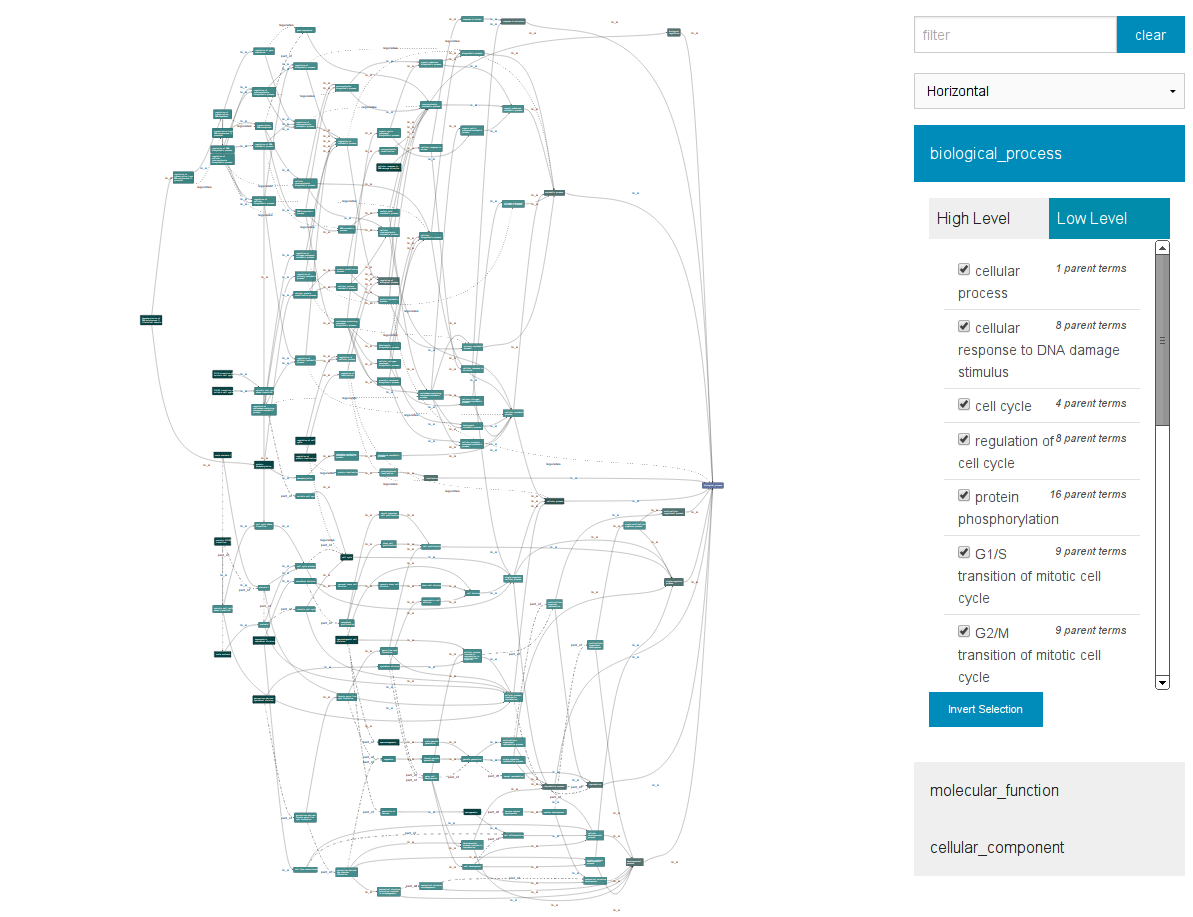
\includegraphics[width=0.4\textwidth]{dagify.png}
\caption{\label{fig:1}The graph viewer, displaying annotations from the gene ontology for the D. melanogaster gene \emph{cdc2}, showing the control panel.}
\end{figure}

\begin{figure}[htb]
\centering
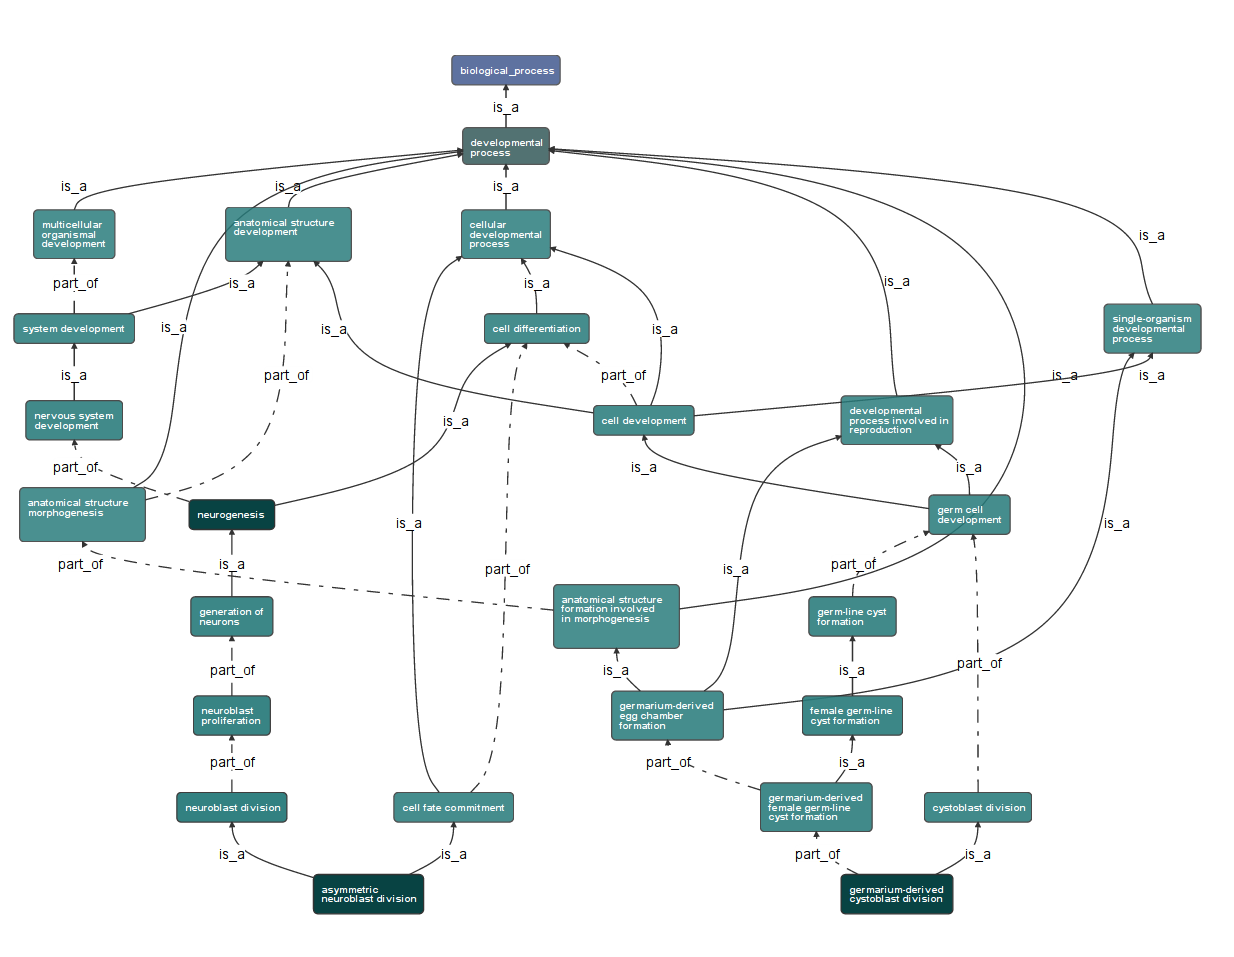
\includegraphics[width=0.4\textwidth]{dagify-subgraph.png}
\caption{\label{fig:2}The graph viewer, displaying a subgraph of annotations from the gene ontology for the D. melanogaster gene \emph{cdc2}, selected using the control panel.}
\end{figure}

The graph viewer presented here uses a collection of publically available, open-source
Javascript tools, including the Backbone~\cite{backbone} framework, the dagre-d3~\cite{dagre-d3}
layout engine, and D3~\cite{d3} data-binding and presentation
library. The combination of these tools make it possible to build a tool in Javascript
and running in modern browsers that provides rich interaction and graphical analysis
possibilities, allowing users to focus on the data, eg. the Gene Ontology Annotation
displayer in figure~\ref{fig:1}.

The current implementation allows a javascript component to be placed on any page
and be provided with any kind of linked network data; the data is rendered
to the screen in the familiar box and line style of a Sugiyama graph drawing. Unlike
static images, this graph can be zoomed, panned, reorientated and rescaled, allowing users to
make sense of dense networks. Since the graph is rendered with SVG technology, rescaling
does not lower graphical resolution, and text legibility is preserved over wide range of zoom
levels.

The user can interact more deeply with this representation than they could with a standard
fixed image. Individual nodes and edges can each have their own styles and behaviour, allowing
contextual tooltips and hover effects to provide information even when zoomed out. Since the
information composing the graph is available to the page at runtime as a data-structure, it can
be searched and filtered, and the graph can been zoomed and scaled to highlight particular nodes
and edges that interest the user.

The graph itself can also be edited at runtime, enabling the ability to display arbitrary 
subgraphs of the main data structure. Figure~\ref{fig:2} illustrates the display of one 
particular subgraph of the information presented in Figure~\ref{fig:1}, reorientated to make the 
best use of the available screen space. This particular subgraph is defined as those nodes 
reachable from one particular high-level ontology term, \emph{developmental process}.

\subsection*{Installation}

As a Javascript tool, installation means indicating which resources a page needs to load.
The DAG viewer tool is a modular javascript component, making use of other
existing resources. As such, the dependencies (appendix~\ref{sec:deps}) need to be included
on the page before the component itself can be used. 
Once these are loaded the BioJS DAGViewer component itself can be included (see code
sample~\ref{code:loading}).
This should be downloaded from the Biojs repository~\cite{site:biojs-registry}
and hosted locally.

\begin{lstlisting}[caption={Loading the DAG-Viewer Library}, label={code:loading}]
<script src="Biojs.DAGViewer.js"></script>
\end{lstlisting}

\subsection*{Usage}

With these elements available, a user is then able to instantiate a new DAG viewer component
pointing at a defined element in the document object model (DOM), or page:

\begin{lstlisting}[caption={Instantiating a new DAGViewer Component}, label={code:new}]
var viewer = new Biojs.DAGViewer({
  target: "element-id"
});
\end{lstlisting}

There is a large number of configurable parameters that can be provided at instantiation
(or indeed, later). These mostly relate to configuring how to interpret the graph data
provided. It is accepted that data may come in different formats, and rather than requiring
users to convert their node and edge data to a predefined format, users can provide adapters
that allow this component to read and display different kinds of graph data, while providing
sensible defaults. More detail is provided on the BioJS registry documentation pages, but as
an example consider a graph (representing a protein interaction network) which has nodes of the form:

\begin{lstlisting}[caption={Example Nodes}, label={code:example-nodes}]
var nodes = [
  {primaryAccession: "P09089", name: "Protein zerknuellt 1"},
  {primaryAccession: "A0ANL0", name: null}
];
\end{lstlisting}

Here we will want to identify each node by its accession number (here from Uniprot) and label
it by its name, if it has one, or by its accession if it does not. This behaviour
cab be defined by passing a couple of parameters:

\begin{lstlisting}[caption={Node Adaptor Example}, label={code:node-adaptor}]
var viewer = new Biojs.DAGViewer({
  target: "element-id",
  nodeLabels: ["name", "primaryAccession"],
  nodeKey: function (n) { return n.primaryAccession; }
});
\end{lstlisting}

Here the \texttt{nodeLabels} parameter indicates which fields should be read to
obtain a label for this node, and the \texttt{nodeKey} parameter is a function that
takes a node and returns an identifier. Similar configuration options exist for
interpreting edges, determining the list of graph roots, providing style classes to
nodes and edges and other functions.

Once configured, the component must be given the definition of the graph it
is meant to visualise. A graph here is defined as two collections, one of nodes,
and the other of edges between nodes. These can be unconnected data structures, such as
loaded from JSON files, without interior references, or they may be circular self-referential
data-structures, with edges pointing to their nodes. A small
graph that represents a (grossly simplified) portion of the \textit{H. sapiens} family tree,
and the viewer to display it, could be configured as follows:

\begin{lstlisting}[caption={\emph{H. sapiens} phylogenetic tree sample graph}]
var species = [
  {name: "H. sapiens", status: "extant"},
  {name: "H. neanderthalensis", status: "extinct"},
  {name: "H. heidelbergensis", status: "extinct"},
  {name: "H. erectus", status: "extinct"},
  {name: "H. ergaster", status: "extinct"},
  {name: "H. habilis", status: "extinct"}
];
var relationships = [
  {subject: species[0], ancestor: species[2]},
  {subject: species[1], ancestor: species[2]},
  {subject: species[2], ancestor: species[4]},
  {subject: species[3], ancestor: species[4]},
  {subject: species[4], ancestor: species[5]}
];
var viewer = new Biojs.DAGViewer({
  target: "element-id",
  nodeLabels: ["name"],
  nodeKey: function (n) { return n.name; },
  edgeProps: ["subject", "ancestor"]
});
viewer.setGraph({
  nodes: species,
  edges: relationships
});
\end{lstlisting}

As well as defining the data model, this component allows applications to respond to
user input. An example of this is responding when a user clicks on a node in the graph. In the
case of our Human ancestry graph, that might look like this:

\begin{lstlisting}[caption={Listening for Events}, label={code:add-listener}]
viewer.addListener(
  "click:node",
  function (name, species) {
    alert(name + " is " + species.get("status"));
  }
);
\end{lstlisting}

\section*{Discussion}

Up to now there have not been any freely available, open-source libraries for efficiently
rendering Sugiyama graph diagrams in the browser. The publication of this library as part of the
Biojs project enables a number of applications that are currently very difficult to implement
correctly. This component is aimed at a need that is particularly relevant for developers in
the life-sciences, where there is frequent need to represent directed graphs, eg.
when dealing with phylogeny, pathways, interactions, developmental stages or ontologies.

Beyond simplifying this task for developers wishing to get started in graphical
network visualisation and analysis, by being built from open web-standard technologies this tool
can be used to interoperate with existing and future applications in ways impossible for static
image rendering tools. The graph definition can be fetched from a remote networked webservice, for
example, thus integrating with a large number of existing browser accessible tools. Because of its
flexible data definition, this component is able to consume data from a wide variety of different
sources with minimal parsing effort. Since the standard node and edge representation is generally
in the form of subject-predicate-object, this component would integrate very well into semantic
web tools serving triples as their data representation.

\section*{Conclusions}
This component meets an important need in the bio-informatics community for an effective,
attractive and usable visualisation tool for a broad variety of directed acyclic graphs.
It is therefore anticipated that this tool will be of use to those developing tools
for researchers in the life-sciences. A great deal of effort has gone into creating,
curating and composing high quality data sets, and there already exist many services which
expose these data-sets to the world through networked web-services. This tool is designed to
plug in seamlessly with existing technologies, helping to maximise the value of existing
and future curated data sets by bringing enhanced visualisation and exploration functionality.
By publishing this component freely
within the Biojs project we expect that a great deal of duplicated
and wasted effort can be avoided, saving significant amounts of time and money for researchers and
their funding bodies.

\subsection*{Competing interests}
The authors declare that there are no competing interests.

\subsection*{Grant information}
InterMine has been developed with the support of the following grants, awarded
to Dr. G. Micklem.

\begin{enumerate}
\item the Wellcome Trust
 \begin{itemize}
 \item{Grant number: 067205}
 \item{Grant number: 082598}
 \item{Grant number: 090297}
 \end{itemize}
\item and the National Human Genome Research Institute.
 \begin{itemize}
 \item{Grant number: R01HG004834}
 \end{itemize}
\end{enumerate}

\nocite{*}
{\small\bibliographystyle{unsrt}
\bibliography{references}}

\clearpage
\section*{Appendix}
\appendix

\section{Dependencies}
\label{sec:deps}

\lstset{language=HTML}
\begin{lstlisting}
<link rel="stylesheet"
      type="text/css"
      href="http://cdn.intermine.org/
css/foundation/5.0/css/foundation.css">
<link rel="stylesheet"
      type="text/css"
      href="http://cdn.intermine.org/js/intermine/dag-viewer/0.0.1-pre/style.css">
<script src="http://cdn.intermine.org/css/foundation/5.0/js/modernizr.js"></script>
<script src="http://cdn.intermine.org/js/jquery/1.9.1/jquery-1.9.1.min.js"></script>
<script src="http://code.jquery.com/ui/1.10.3/jquery-ui.js"></script>
<script charset="UTF-8" src="http://cdn.intermine.org/js/intermine/dag-viewer/0.0.1-pre/index.js">
<script src="http://cdn.intermine.org/css/foundation/5.0/js/foundation/foundation.js"></script>
\end{lstlisting}

Note that the foundation scripts at least must be loaded in the
\texttt{body} section of the HTML page, since they require the
Document Object Model (DOM) to be ready before they can be loaded.

% See this guide for more information on BibTeX:
% http://libguides.mit.edu/content.php?pid=55482&sid=406343

% For more author guidance please see:
% http://f1000research.com/author-guidelines


% When all authors are happy with the paper, use the 
% ‘Submit to F1000Research' button from the Share menu above
% to submit directly to the open life science journal F1000Research.

% Please note that this template results in a draft pre-submission PDF document.
% Articles will be professionally typeset when accepted for publication.

% We hope you find the F1000Research writeLaTeX template useful,
% please let us know if you have any feedback using the help menu above.


\end{document}
